\section{Experiments}
\label{sec:exp}

In this section, we first describe our dataset and how we preprocess it. We
then introduce all baselines and evaluation metrics. Finally, we present
our research questions and results.

\subsection{Data Collection}
\label{sec:data}

We take our data from the patches that have been committed to mainline
Linux
kernel\footnote{git://git.kernel.org/pub/scm/linux/kernel/git/torvalds/linux.git}
v3.0, released in July 2011, through v4.12, released in July 2017.  We
additionally collect information from the stable
kernels\footnote{git://git.kernel.org/pub/scm/linux/kernel/git/stable/linux.git}
that had been released as of October 2017 building on Linux kernels v3.0
through v4.13.  We consider mainline commits that are duplicated in at
least one stable version to be stable-relevant.  We also consider mainline
commits to so-called ``release candidates'', that are predecessors to a
mainline kernel release, to be stable-relevant when such commits are to a
release candidate that is after the first one for a given version.  Indeed,
commits to these release candidates are expected to contain only bug fixes
and they can be viewed as the stable
versions of the new features proposed in the first release
candidate.  We refer to patches that are propagated to stable kernels or
are found in later release candidates as {\em stable patches} and patches
that are not propagated to stable kernels or found in later release
candidates as {\em non stable patches}.  To avoid biasing the learning
process towards either stable or non stable patches, we construct our
datasets such that the number of patches in each category is roughly
balanced.  While this situation does not reflect the number of stable and
non stable patches that confront a stable kernel maintainer each day, it
allows effective training and interpretation of the experimental results.

\subsubsection{Identifying Stable Patches}
\label{sec:stable_patch}

The main challenge in constructing the datasets is to determine which
mainline patches have been propagated to stable kernels.  Indeed, there is
no required link information connecting the two.  Some stable patches
explicitly mention the corresponding mainline commit in the commit message,
which we refer to as a {\em back link}. For others, we rely on the author
name and the subject line. Subject lines typically contain information
about both the change made and the name of the file or directory in which
the change is made, and thus should be unique.  Accordingly, we first
collect from the patches in the stable kernels a list of any back
links and a list of pairs of author name and subject line.  A commit from
the mainline whose commit id is mentioned in a back link or whose author
name and subject line are the same as one found in a patch to a stable
kernel is considered to be a stable-relevant patch.

\subsubsection{Collecting the dataset}
\label{sec:mainline_patch}

We collect our dataset from the mainline kernel.  In order to focus on
patches that are challenging for stable maintainers to classify, we drop in
advance all patches that do not meet the stable-kernel size
guidelines,\footnote{https://www.kernel.org/doc/html/v4.15/process/stable-kernel-rules.html}
{\em i.e.}, those that exceed 100 code lines, including both changed lines
and its context as reported by the {\tt diff} command.  We then keep all
identified stable patches for our dataset and select an equal number of non
stable patches.  When possible, we select non stable patches that have a
similar number of changed lines as the stable patches, again to create a
dataset that reflects the cases that cannot be excluded by size alone and
thus are challenging for stable kernel maintainers.  These patches are then
subject to a preprocessing step that is detailed in the next section.

Our dataset comes from Linux kernel mainline versions 3.0 (July 2011)
through 4.12 (July 2017). There were 424,380 commits during that period.  We
consider only those commits that are not merge commits, that modify a file
as opposed to only adding or removing files, and that affect at least one
{\tt .c} or {\tt .h} file.  This leaves 346,570 commits (82\%).  Of these
346,570 commits, 79,319 (23\%) are not considered because they contain more
than 100 changed lines, leaving 267,251 commits.  Of these, we pick the
42,408 stable patches for which the preprocessing step is successful and
39,995 non-stable patches, {\em i.e.}, 82,403 patches in all.

%82597 (training) + 122,364 = 204,961 commits.  The 82,597 commits include
%all commits that have been applied to stable trees and that are in "rc"
%(release candidate) versions between rc1 and the subsequent version.  The
%commits up to rc1 are primarily adding new features, whereas the commits
%in the subsequent release candidates should increasingly consist of only
%bug fixes on the recently added features.

%In general, our training set is noisy.  Most of our stables should be bug
%fixes, but a small percentage of stables may be there for other reasons,
%such as that a bug fix depends on them or that they add a new device
%identifier that is considered to be trivial and useful enough to be worth
%making a modification to a stable version.  The whole point of our work is
%that there may be stable relevant patches the maintainers are not
%currently marking as stable and that are thus getting overlooked.  If we
%can run the algorithm on the larger dataset, then we can evaluate whether
%our approach compensates for the laziness of maintainers, by highlighting
%more patches of maintainers who are currently underreporting. But
%currently, we have no way to show that we do better than current practice.

\subsection{Patch Preprocessing}
\label{sec:patch_processing}

Our approach applies some preprocessing steps to the patches before they are
given to PatchNet.

\subsubsection{Preprocessing of commit messages}

Our approach applies various standard natural language techniques to the
commit messages, such as stop word elimination and
stemming~\cite{vijayarani2015preprocessing, brants2003natural}, to reduce
message length and eliminate irrelevant information.  Subsequently, we pad
or truncate all commit messages to the same size, specifically 512 words,
covering the complete commit message for all but two patches, for
parallelism.  Because we are interested in cases that are challenging for
the stable kernel maintainer, we drop tags such as Cc: stable and Fixes,
whose goal is to indicate that a given patch is a stable-relevant or a bug
fixing patch.  We also drop tags indicating who has approved the patch, as
the set of developers and their work profiles can change in the future.

\subsubsection{Preprocessing of code changes}
\label{sec:extract_level_diff}

Diff code elements, as illustrated in Figure~\ref{fig:sample_patch}, may
have many shapes and sizes - from a single word to multiple lines spread
out over multiple hunks. To describe changes in terms of meaningful
syntactic units and to provide context for very small changes, we collect
differences at roughly the granularity of atomic statements. These may be,
{\em e.g.}, simple assignment statements, return statements, if headers,
etc.  For example, in the patch illustrated in
Figure~\ref{fig:sample_patch}, the only change is to replace {\tt 1} on
line 22 by {\tt err} on line 23.  Nevertheless, we represent the change as
a change in the complete return statement, {\em i.e.}, {\tt return 1;} is
transformed into {\tt return err;}.  We also distinguish changes in error
checking code (code to detect whether an error has occurred, {\em e.g.}, line
21 in Figure~\ref{fig:sample_patch}) and in error handling code (code to
clean up after an error has occurred, {\em e.g.}, lines 22 and 23 in
Figure~\ref{fig:sample_patch}) from changes in other code, which we refer
to as {\em normal code}. Error checking code and error handling code are
indeed very common in the Linux kernel, which must be robust, and they are
disjoint in structure and purpose from the implementation of the main
functionality.

For a given commit, the first step is to extract the names of the affected
files and to extract the state of those files before and after the
commit. Analogous to the stemming and stop word elimination performed at
the commit message level, for each before and after file instance, we
remove comments and the contents of strings, as changes in comments and
within strings are not likely to be stable-relevant. For a given pair of
before and after files, we then compute the difference using the command
``git diff -U0 old new'', giving the changed lines with no lines of
% * <hvdthong@gmail.com> 2018-08-25T10:47:15.001Z:
%
% ^.
% * <hvdthong@gmail.com> 2018-08-25T10:47:13.368Z:
%
% ^.
surrounding context. For each ``--'' or ``+'' line in the diff output, we
then collect a record indicating the sign (``--'' or ``+''), the category
(error-handling code, etc.), the hunk number, the line number in the old or
new version, respectively, and the starting and ending columns of the
non-space changes on the line.  We furthermore keep the names of called
functions, when these are not defined in the same file and are used at
least 5 times, but drop other identifiers, {\em i.e.} field names and
variable names, as these may be too diverse to allow effective learning and unnecessarily slow down the training time.
Indeed, adding just the frequently used function names increases the code
vocabulary size from 43 to 3,616 unique tokens, which
increases the training time.

To extract changes at the level of atomic statements, rather than the
individual lines obtained by diff, we parse each file as it exists before
and after the change and keep the atomic statements that intersect with
a changed line observed by diff.  For this, we use the parser of the C
program transformation system Coccinelle~\cite{padioleau2008documenting},
which uses heuristics to parse around compiler directives and macros
\cite{yoann:cc}.  This makes it possible to reason about patches in terms
of the way they appear to the user, without macro expansion, but comes with
some cost, as some patches must be discarded because the parsing heuristics
are not sufficient to parse all of the code affected by the changed
lines. %\jl{Perhaps some numbers should appear here}

By following the above-mentioned steps, we collect the affected files of a
given patch. For each removed or added code line of the affected file,
denoted by ``--'' and ``+'', we collect a hunk number and a line number
corresponding to the removed or added code line. Each word in a line is a
pair of the associated token and the annotation indicating whether the word
occurs on a line of as error-checking code, error-handling code, or normal
code.  This information is used to build the two three-dimensional matrices
representing the removed code and the added code for the affected file
({\em cf.} Figure \ref{fig:commit_code_model}).

\subsection{Baselines}
\label{sec:baselines}
We compare PatchNet with several baselines:

\begin{itemize}[leftmargin=0.4cm]
\item Keyword: As a simple but frequently used
  heuristic~\cite{tian2012identifying}, we select all commits in which the
  commit message includes ``bug'', ``fix'', or ``bug-fix'' after conversion
  of all words to lowercase and stemming.  While not all bug fixes are
  relevant for stable kernels, as some bugs may have very low impact or the
  fix may be too large or complicated to be considered clearly correct, the
  problem of identifying bug fixes is close enough to that of recognizing
  stable relevant patches to make comparison with our model valuable.
\item LPU+SVM: This method for identifying bug-fixing patches was proposed
  by Tian et
  al.~\cite{tian2012identifying} and comprises two algorithms, i.e.,
  Learning from Positive and Unlabeled Examples
  (LPU)~\cite{joachims1999svmlight, letouzey2000learning, liu2003building}
  and Support Vector Machine (SVM)~\cite{cauwenberghs2001incremental,
    cristianini2000introduction}, which are used to build a classification
  model for automatically identifying bug fixing patches. The set of code
  features considered was manually selected. In Tian et al.'s work, stable kernels were
  considered as a source of bug-fixing patches in the training and testing
  data.

 \item LS-CNN: Huo et al.~\cite{huo2017enhancing} combined
   LSTM~\cite{hochreiter1997long} and CNN~\cite{lecun1998gradient} 
%    \jl{Could LSTM be mentioned first, since the name of the approach is
%      LS-CNN?} \jg{I'll fix it then} 
     to localize potential buggy source files based on bug report
   information. They used CNN to learn a representation of the bug report
   and a combination of LSTM and CNN 
%    \jl{again, could LSTM be mentioned
%      first?} 
     to learn the structure of the code.  To assess the ability of
   LS-CNN to classify patches as stable relevant, for a given patch, we
   give the commit message as input to LS-CNN in place of the bug
   report and the result of concatenating the lines changed in the various
   files and hunks as input to LS-CNN in place of the potential buggy
   source file.
  
% \jh{Comment 7: Missing vital references and related work discussions to justify novelty of PatchNet compared to other baselines (i.e., LSTM-CNN or LPU-SVM). Why should we choose CNN over LSTM or RNN? (reviewer B, meta reviewer)}

% \jg{Julia: I already rewrote the paragraph LS-CNN, can you please check it
%   out again?}
% \jl{I rewrote the above paragraph}

\item Feed-Forward Fully Connected Neural Network (F-NN): Inspired by the
  above-cited work of Tian et al.\ on LPU+SVM, a Linux stable kernel
  maintainer, Sasha Levin, has developed an approach to identifying
  stable patches \cite{sasha} based on a Feed-Forward Fully
  Connected Neural Network~\cite{bishop1995neural, goodfellow2016deep} and
  a set of manually selected features, including frequent commit message
  words, author names, and some code metrics.  Levin actively uses this
  approach in his work on the Linux kernel.
\end{itemize}

For LPU-SVM and LS-CNN, we used the same parameters and settings as
described in the respective papers. For F-NN, we asked Levin to train the tool on our training data and
test it with our testing data. We use 50\% as the cut off for considering a patch to be stable relevant for PatchNet and all baselines.

\subsection{Training and hyperparameters}
\label{sec:parameters}

%We empirically run PatchNet on different the number of convolutional filters and number of convolutional filter length and select the best number of convolutional filters and filter length for our model. %(i.e., $k=1$ and $k=2$) having length 64 on both \textit{commit message module} and \textit{commit code module} for training PatchNet. 

% PatchNet also has a number of other hyperparameters. 
% We set the size of PatchNet's hidden layer ($\textbf{h}$), $l_2$ regularization, and the dropout rate to be 100, $1e-5$, and 0.5, respectively. The dimensions of
% the word vectors in commit message $d_m$ and code changes $d_c$ are set to
% 50. PatchNet is trained using SGD~\cite{bottou2010large} with shuffled
% mini-batches. The batch size is set to 32. We train PatchNet for 25 epochs
% and apply the early stopping strategy~\cite{prechelt1998automatic}, i.e.,
% we stop the training if there has been no update to the loss value (see Equation~\ref{eq:cost}) for the last 5 epochs. These parameters follow a prior work~\cite{severyn2015learning}. 

% The parameters \jl{hyperparameters?} of PatchNet were chosen as follows:
% the number of convolutional filters, the size of PatchNet's hidden layer
% ($\textbf{h}$), $l_2$ regularization \jl{I don't understand what is the
%   parameter here}, and the dropout rate to be 64, 100, $1e-5$, and 0.5,
% respectively \jl{This is hard to read - the respectively is too complex.
%   Just give the numbers one by one.  Or consider making a table.}. The
% dimensions of the word vectors in commit message $d_m$ and code changes
% $d_c$ are set to 50. PatchNet is trained using SGD~\cite{bottou2010large}
% \jl{I thought we use Adam, which is different than SGD.} with shuffled
% mini-batches. The batch size is set to 32. We train PatchNet for 25 epochs
% and apply the early stopping strategy~\cite{prechelt1998automatic}, i.e.,
% we stop the training if there has been no update to the loss value (see
% Equation~\ref{eq:cost}) for the last 5 epochs. All these parameters of our
% model are in line with a prior work~\cite{severyn2015learning, yu2014deep}.

% \jh{Comment 8: Hyper-parameters: how do we select parameters for deep learning models? (reviewer C, meta reviewer)}

% \jg{Julia: can you please check this section?}

For the sizes of the filters described in Section~\ref{sec:approach}, we choose $k \in \{1, 2\}$, making the associated
windows analogous to a 1-gram or 2-gram as used in natural language
processing~\cite{jurafsky2014speech, brown1992class}. 
% \ty{I move this
%   paragraph from the approach section to here because it is a
%   parameter. Please add it to the above parameter list.} 
  Using 2-grams
allows our approach to take into account the temporal ordering of words,
going beyond the bag of words used by Tian et
al.~\cite{tian2012identifying}. The number of convolutional filters is set
to 64. The size of the fully-connected layer described in Section~\ref{sec:classification_model} is set to 100. The
dimensions of the word vectors in commit message $d_m$ and code changes
$d_c$ are set to 50. PatchNet is trained using Adam~\cite{kingma2014adam}
% \jl{I thought we use Adam, which is different than SGD.} 
with shuffled
mini-batches. The batch size is set to 32. We train PatchNet for 25 epochs
and apply the early stopping strategy~\cite{prechelt1998automatic, caruana2001overfitting}, i.e.,
we stop the training if there has been no update to the loss value (see
Equation~\ref{eq:cost}) for the last 5 epochs. All these hyperparameter values
% parameters
% \jl{hyperparameter values?}
are widely used in the deep learning community~\cite{severyn2015learning, huo2016learning, huo2017enhancing, hinton2012improving}. 
% in line with a prior work~\cite{severyn2015learning}.  

%Note that the word embedding matrices are learned during the training process. 

% ~\cite{mou2016convolutional}. 

\subsection{Evaluation Metrics}
\label{sec:metrics}
To evaluate the effectiveness of a stable patch identification
model, we employ the following metrics:

\begin{itemize}[leftmargin=0.4cm]
\item Accuracy: Proportion of stable and non-stable patches that are correctly classified.
\item Precision: Proportion of patches that are correctly classified as stable. 
\item Recall: Proportion of stable patches that are correctly classified. 
\item F1: Harmonic mean between precision and recall
\item AUC: Area under the Receiver Operating Characteristic curve. It measures if the stable patches tend to have higher predicted probabilities (to be stable) than non stable ones. 
\end{itemize}

% decision tree (DTree)~\cite{safavian1991survey}, long short-term memory (LSTM)~\cite{hochreiter1997long}, birectional long short-term memory (Bi-LSTM)~\cite{graves2005bidirectional}, convolutional neural network (CNN)~\cite{kim2014convolutional}, 

\subsection{Research Questions and Results}
\label{sec:rq}
Our study seeks to answer three research questions: 

\vspace{0.1cm}\noindent{\bf RQ1: How to decompose the dataset into training
  and testing data?}  A common strategy for evaluating machine learning
algorithms is $n$-fold cross-validation~\cite{kohavi1995study},
in which a dataset is randomly distributed among $n$ equal-sized buckets,
each of
which is considered as test data for a model trained on the contents of the
remaining $n-1$ buckets.  When data elements become available over time, as
is the case of Linux kernel patches, this strategy can result in testing a
model on data that predates some of the data on which the model was
trained.  Respecting the order in which patches are submitted,
however, would limit the amount of testing that can be done, given
the fairly small number of stable patches available.

To address this issue, we first assess whether training on future data
helps or harms the accuracy of PatchNet on our dataset.  We first sort the
patches collected in Section~\ref{sec:data} from earliest to latest based
on the date when the patch author submitted the patch to maintainers. Then,
we divide the dataset into 5 mutually exclusive sets by date. Note that the
resulting five sets are not perfectly balanced, but they come close, with
stable patches making up 45\% to 55\% of each set.  Then, we repeat the
following process five times: take one set as a testing set and use the
remaining four sets for training. When we test on the first set, we observe
the impact of training only on future data.  When we test on the fifth set,
we observe the impact of training only on past data.  The other testing
sets use models trained on a mixture of past and future data.

Table~\ref{tab:cross_valid_patchnet} shows the results of PatchNet on the
different test sets. The standard deviations are quite small (i.e., below
0.013), hence there is no difference between training on past or future
data.  Our dataset starts with Linux v3.0, which was released in 2011,
twenty years after the start of work on the Linux kernel.  The lack of
impact due to training on past or future data suggests that in such a
mature code base the properties that make a patch relevant for stable
kernels are fairly constant over time.  This property is indeed beneficial,
because it means that our approach can be used to identify stable-relevant commits that have been missed in older versions.  In subsequent research
questions, we thus retain the same five test and training sets.

\begin{table}[t!]
  \centering
  \caption{The results of PatchNet on the five chronological
    test sets}
    \begin{tabular}{|l|c|c|c|c|c|}
    \hline
          & \textbf{Accuracy} & \textbf{Precision} & \textbf{Recall} & \textbf{F1}    & \textbf{AUC} \\
    \hline
    \hline
    Set=1 & 0.852 & 0.841 & 0.886 & 0.863 & 0.850 \\
    \hline
    Set=2 & 0.860  & 0.833 & 0.909 & 0.869 & 0.859 \\
    \hline
    Set=3 & 0.866 & 0.833 & 0.910  & 0.870  & 0.867 \\
    \hline
    Set=4 & 0.864 & 0.828 & 0.912 & 0.868 & 0.864 \\
    \hline
    Set=5 & 0.869 & 0.860  & 0.917 & 0.887 & 0.862 \\
    \hline
%     \textbf{Average} & \textbf{0.862} & \textbf{0.839} & \textbf{0.907} & \textbf{0.871} & \textbf{0.860} \\
    \hline
    \textbf{Std.} & \textbf{0.007} & \textbf{0.013} & \textbf{0.012} & \textbf{0.009} & \textbf{0.007} \\
    \hline
    \end{tabular}%
  \label{tab:cross_valid_patchnet}%
\end{table}%

\vspace{0.1cm}\noindent{\bf RQ2: How effective is PatchNet compared to
  other state-of-the-art stable patch identification models?}  To
answer this RQ, we use the five copies of the dataset described in RQ1. At
the end of the 5 iterations, we collect the results to get the aggregated
accuracy, precision, recall, F1, and AUC scores.
Table~\ref{tab:msg_code}
shows the results for PatchNet as well as the other baselines. We see that
PatchNet achieves accuracy, precision, recall, F1, and AUC scores of 0.862,
0.839, 0.907, 0.871, and 0.860, respectively. Comparing them to the best
performing baseline (i.e., F-NN), these constitute improvements of
6.55\%, 0.12\%, 16.13\%, 7.80\%, and 6.30\% in terms of accuracy,
precision, recall, F1, and AUC scores, respectively. PatchNet thus achieves
about the same precision as F-NN, but a significant improvement in terms of
recall. This is achieved without the feature engineering required to
implement the F-NN approach, but rather by automatically learning the weight of the filters
via our hierarchical deep learning-based architecture.

\begin{table}[t!]
  \centering
  \caption{PatchNet vs. Keyword, LPU+SVM, LS-CNN, and F-NN.}
    \begin{tabular}{|l|c|c|c|c|c|}
    \hline
          & \textbf{Accuracy} & \textbf{Precision } & \textbf{Recall} & \textbf{F1} & \textbf{AUC} \\
    \hline
    \hline
    Keyword & 0.626 & 0.683 & 0.515 & 0.587 & 0.630 \\
    \hline
    LPU+SVM & 0.731 & 0.751 & 0.716 & 0.733 & 0.731 \\
%     \hline
%     DTree & 0.637 & 0.649 & 0.649 & 0.649 & 0.637 \\
%     \hline
%     LSTM  & 0.675 & 0.690  & 0.673 & 0.681 & 0.675 \\
%     \hline
%     Bi-LSTM & 0.677 & 0.688 & 0.689 & 0.688 & 0.677 \\
%     \hline
%     CNN   & 0.66  & 0.679 & 0.650  & 0.664 & 0.661 \\
    \hline
    LS-CNN & 0.765 & 0.766 & 0.785 & 0.775 & 0.765 \\
    \hline
    F-NN & 0.809 & 0.838 & 0.781 & 0.808 & 0.809 \\
    \hline
    PatchNet & \textbf{0.862} & \textbf{0.839} & \textbf{0.907} & \textbf{0.871} & \textbf{0.860} \\
    \hline
    \end{tabular}%
  \label{tab:msg_code}%
\end{table}%

% Figure~\ref{fig:prc_rc_curve} shows a precision-recall curve of PatchNet
% and the baselines. For a given precision, PatchNet obtains the highest
% recall, and for a given recall, PatchNet obtains the highest precision. 

% Figure~\ref{fig:prc_rc_curve} shows a precision-recall curve of PatchNet
% and the baselines. Pegging precision at [0.95-1.0] range, PatchNet can achieve a recall in the [0.786-0.524], while the best performing baseline can only achieve a recall of [0.684-0.514]. This translates to a [14.91\%, 1.95\%] improvement of precision. Similarly pegging recall at [0.95-1.0] range, PatchNet can achieve a recall in the [0.603-0.0], while the best performing baseline can only achieve a recall of [0.427-0.181]. This translates to a [41.22\%, -] improvement.

Figure~\ref{fig:prc_rc_curve} compares the precision-recall curves for
PatchNet and the baselines. For most values
on the curve, PatchNet obtains the highest recall for a given precision; as well as the highest precision for a given recall. For example, considering a low false positive rate of 5 percent (precision of 0.95), PatchNet achieves a recall of 0.786 which is 14.9\% higher than that of the best performing baseline. Likewise, considering a low false negative rate of 5 percent (recall of 0.95), PatchNet achieves a precision of 0.603 which is 41.2\% higher than that of the best performing baseline. In addition, considering the sweet spots where both precision and recall are high (larger than 0.8), PatchNet can achieve a F1 of up to 0.886 which is 10.6\% higher than that of the best performing baseline.
% \ty{modified, need verify the numbers, 10.61\% not 29.8\% right?} \jg{correct}

%Additionally, considering the sweet spots where both precision and recall are high, PatchNet can achieve a harmonic mean of precision and recall (F1) of up to 0.684 which is 29.80\% higher than that of the best performing baseline. 


%Figure~\ref{fig:prc_rc_curve} shows a precision-recall curve of PatchNet and the baselines. At lower recall level (up to 50\%), all the approaches performed similarly. However, as the recall level increased to 80\%, the precisions of baseline approaches dropped by 20-20\% while PatchNet remains a high precision of 0.9. Figure~\ref{fig:prc_rc_curve} also shows that along the precision-recall curve, for a given precision, PatchNet obtains the highest recall, and for a given recall, PatchNet obtains the highest precision. 


Figure~\ref{fig:venn_diagram} shows Venn diagrams indicating the number of patches that PatchNet and each of the baselines correctly recognize as stable-relevant. The top diagram compares the Keyword approach to the two approaches, PatchNet and LS-CNN, that automatically learn the relevant features.  While there are over 20K patches in common that all three approaches classify as stable-relevant, there are another 11K that are
found by both learning-based approaches, showing the advantage of
learning-based approach.  PatchNet furthermore correctly detects over 3x
more stable-relevant patches than LS-CNN, showing the value of an approach
that takes the properties of code changes into account.  The bottom diagram
then compares PatchNet to the two approaches, LPU+SVM and F-NN, in which
the code features are hand crafted.  While all three approaches correctly
recognize over 27K patches as stable-relevant, there are again 3x more
patches that only PatchNet correctly detects as stable-relevant than there
are that only each of the other two approaches recognizes as stable-relevant.

\begin{figure}
\centering
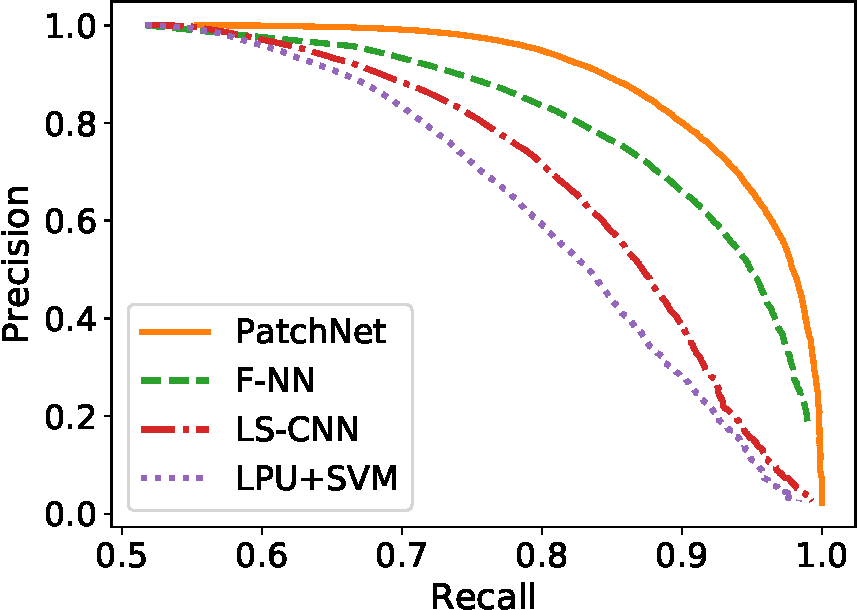
\includegraphics[scale=0.375]{figures/prc_recall_curve_ver1.pdf}
	\caption{Precision-recall curve: PatchNet vs. LPU+SVM, LS-CNN, and F-NN.}
	\label{fig:prc_rc_curve}
    \vspace{-0.4cm}
\end{figure}

% \begin{figure}
% % \centering
% % 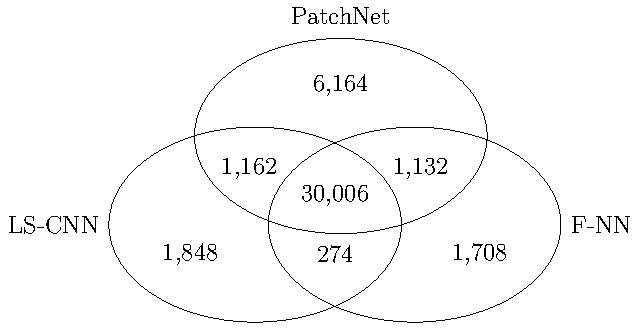
\includegraphics[scale=0.45]{figures/ven_diagram_ver1.pdf}
% % 	\caption{A Venn diagram showing overlapping of stable patches in three different algorithms, i.e., PatchNet, F-NN, and LS-CNN.}
% % 	\label{fig:venn_diagram}
% %     \vspace{-0.4cm}
% \def\first{(-.2,0) ellipse (6em and 3em)}
% \def\second{(1,0) ellipse (6em and 3em)}
% \def\third{(0.4,0.5) ellipse (6em and 3em)}
% \centerline{\begin{tikzpicture} \scriptsize
%     \draw \first node [below] (An) {};
%     \draw \second node [below] (Bn) {};
%     \draw \third node [above] (Cn) {};
% %
%     % first coordinate control x axis, second controls y axis
%     \node at (-1.1,-.2) (A) {1,848};
%     \node at (1.9,-.2) (B) {1,708};
%     \node at (.4,.95) (C) {6,164};
% %
%     \node at (.4,.2) {30,006};
% %
%     \node at (.4,-.4) {274}; % LS-CNN and F-NN
%     \node at (-0.65,.4) {1,162}; % LS-CNN and PatchNet
%     \node at (1.45,.4) {1,132}; % F-CNN and PatchNet
% %
%     \node[anchor=east] at (-1.7,0) {LS-CNN};
%     \node[anchor=west] at (2.5,0) (B) {F-NN};
%     \node[anchor=south] at (0.4,1.3) (C) {PatchNet};
% %
%   \end{tikzpicture}}
% 	\caption{A Venn diagram showing overlapping of stable patches in three different algorithms, i.e., PatchNet, F-NN, and LS-CNN.}
% 	\label{fig:venn_diagram}
% \end{figure}

\begin{figure}
\def\firsta{(-.2,0) ellipse (6em and 3em)}
\def\seconda{(1,0) ellipse (6em and 3em)}
\def\thirda{(0.4,0.5) ellipse (6em and 3em)}
\centerline{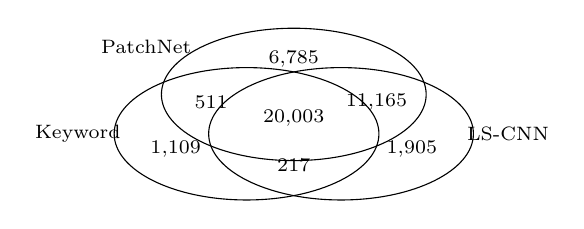
\begin{tikzpicture} \scriptsize
    \draw \firsta node [below] (An) {};
    \draw \seconda node [below] (Bn) {};
    \draw \thirda node [above] (Cn) {};
%
    % first coordinate control x axis, second controls y axis
    \node at (-1.1,-.2) (A) {1,109};
    \node at (1.9,-.2) (B) {1,905};
    \node at (.4,.95) (C) {6,785};
%
    \node at (.4,.2) {20,003};
%
    \node at (.4,-.4) {217}; % LS-CNN and F-NN
    \node at (-0.65,.4) {511}; % LS-CNN and PatchNet
    \node at (1.45,.4) {11,165}; % F-CNN and PatchNet
%
    \node[anchor=east] at (-1.7,0) {Keyword};
    \node[anchor=west] at (2.5,0) (B) {LS-CNN};
    \node[anchor=east] at (-.8,1.1) (C) {PatchNet};
%
  \end{tikzpicture}}

\vspace{\baselineskip}

\def\first{(-.2,0) ellipse (6em and 3em)}
\def\second{(1,0) ellipse (6em and 3em)}
\def\third{(0.4,0.5) ellipse (6em and 3em)}
\centerline{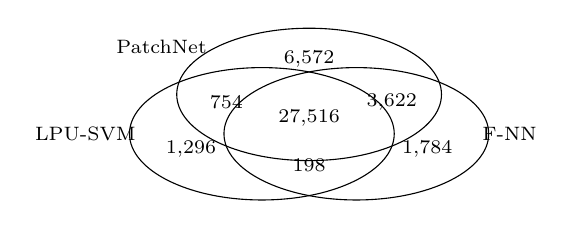
\begin{tikzpicture} \scriptsize
    \draw \first node [below] (An) {};
    \draw \second node [below] (Bn) {};
    \draw \third node [above] (Cn) {};
%
    % first coordinate control x axis, second controls y axis
    \node at (-1.1,-.2) (A) {1,296};
    \node at (1.9,-.2) (B) {1,784};
    \node at (.4,.95) (C) {6,572};
%
    \node at (.4,.2) {27,516};
%
    \node at (.4,-.4) {198}; % LS-CNN and F-NN
    \node at (-0.65,.4) {754}; % LS-CNN and PatchNet
    \node at (1.45,.4) {3,622}; % F-CNN and PatchNet
%
    \node[anchor=east] at (-1.7,0) {LPU-SVM};
    \node[anchor=west] at (2.5,0) (B) {F-NN};
    \node[anchor=east] at (-.8,1.1) (C) {PatchNet};
%
  \end{tikzpicture}}
	\caption{Venn diagrams showing the number of stable
          patches identified by PatchNet and the various baselines}
	\label{fig:venn_diagram}
\end{figure}

\vspace{0.1cm}\noindent{\bf RQ3: Does PatchNet benefit from considering
  both the commit message and the code changes, and do function names help
  identify stable patches?}  To answer this RQ, we conduct an ablation
test~\cite{korbar2017deep, liu2017deep}
% \jg{recheck refs} 
by ignoring the
commit message, the code changes, or the function names in the code changes
in a given patch one-at-a-time and evaluating the performance. We create
three variants of PatchNet: PatchNet-C, PatchNet-M, and
PatchNet-NN. PatchNet-C uses only code change information while PatchNet-M
uses only commit message information. PatchNet-NN uses both code change and
commit message information, but ignores the function names in the code
changes. We again use the five copies of the dataset described in RQ1 and
compute the various evaluation metrics.

Table~\ref{tab:components} shows that the performance of PatchNet degrades
if we ignore any one of the considered types of information. Accuracy,
precision, recall, F1, and AUC drop by 19.39\%, 15.41\%, 21.26\%, 18.34\%,
and 16.06\% respectively if we ignore commit messages. They drop by 16.96\%,
14.62\%, 16.58\%, 14.76\%, and 14.21\% respectively if we ignore code
changes.  And they drop by 11.08\%, 12.62\%, 16.43\%, 13.86\%, and 11.98\%
respectively if we ignore function names.  Thus, each kind of information
contributes to PatchNet's performance.  Additionally, the drops are
greatest if we ignore commit messages, indicating that they are slightly
more important than the other two to PatchNet's performance.

\begin{table}[t!]
  \centering
  \caption{Contribution of commit messages and code changes to PatchNet's performance}
    \begin{tabular}{|l|c|c|c|c|c|}
    \hline
          & \textbf{Accuracy} & \textbf{Precision} & \textbf{Recall} & \textbf{F1}    & \textbf{AUC} \\
    \hline
    \hline
    PatchNet-C & 0.722 & 0.727 & 0.748 & 0.736 & 0.741 \\
    \hline
    PatchNet-M & 0.737 & 0.732 & 0.778 & 0.759 & 0.753 \\
    \hline
    PatchNet-NN & 0.776 & 0.745 & 0.779 & 0.765 & 0.768 \\
    \hline
    PatchNet & \textbf{0.862} & \textbf{0.839} & \textbf{0.907} & \textbf{0.871} & \textbf{0.860} \\
    \hline
    \end{tabular}%
  \label{tab:components}%
\end{table}%

% % Table generated by Excel2LaTeX from sheet 'Sheet5'
% \begin{table}[t!]
%   \centering
%   \caption{CODE}
%     \begin{tabular}{|l|c|c|c|c|c|}
%     \hline
%           & Accuracy & Precision & Recall & F1    & AUC \\
%     \hline
%     \hline
%     BugFix & -     & -     & -     & -     & - \\
%     \hline
%     LPU-SVM & 0.649 & 0.817 & 0.571 & 0.672 & 0.676 \\
%     \hline
%     LS-CNN & 0.726 & 0.829 & 0.69  & 0.753 & 0.754 \\
%     \hline
%     PatchNet & \textbf{0.769} & \textbf{0.859} & \textbf{0.697} & \textbf{0.77} & \textbf{0.752} \\
%     \hline
%     \end{tabular}%
%   \label{tab:code}%
% \end{table}%

% \begin{table}[t!]
%   \centering
%   \caption{CODE}
%     \begin{tabular}{|l|c|c|c|c|c|}
%     \hline
%           & \textbf{Accuracy} & \textbf{Precision } & \textbf{Recall } & \textbf{F1} & \textbf{AUC} \\
%     \hline
%     \hline
%     BugFix & -     & -     & -     & -     & - \\
%     \hline
%     LPU+SVM & -     & -     & -     & -     & - \\
%     \hline
%     DTree & 0.561 & 0.574 & 0.583 & 0.578 & 0.56 \\
%     \hline
%     LSTM  & 0.584 & 0.568 & 0.821 & 0.671 & 0.576 \\
%     \hline
%     Bi-LSTM & 0.577 & 0.570  & 0.741 & 0.644 & 0.571 \\
%     \hline
%     CNN   & 0.579 & 0.570  & 0.757 & 0.650  & 0.573 \\
%     \hline
%     LSTM-CNN & 0.583 & 0.574 & 0.748 & 0.649 & 0.577 \\
%     \hline
%     PatchNet & \textbf{0.654} & \textbf{0.675} & \textbf{0.719} & \textbf{0.696} & \textbf{0.655} \\
%     \hline
%     \end{tabular}%
%   \label{tab:code}%
% \end{table}%

% \begin{table}[t!]
%   \centering
%   \caption{Add caption}
%     \begin{tabular}{|l|c|c|c|c|c|}
%     \hline
%           & \textbf{Accuracy} & \textbf{Precision } & \textbf{Recall } & \textbf{F1} & \textbf{AUC} \\
%     \hline
%     \hline
%     BugFix & 0.626 & 0.683 & 0.515 & 0.587 & 0.63 \\
%     \hline
%     LPU+SVM & -     & -     & -     & -     & - \\
%     \hline
%     DTree & 0.64  & 0.653 & 0.649 & 0.651 & 0.64 \\
%     \hline
%     LSTM  & 0.672 & 0.68  & 0.689 & 0.684 & 0.671 \\
%     \hline
%     Bi-LSTM & 0.668 & 0.698 & 0.629 & 0.661 & 0.669 \\
%     \hline
%     CNN   & 0.678 & 0.686 & 0.695 & 0.691 & 0.678 \\
%     \hline
%     LSTM-CNN & 0.668 & 0.698 & 0.629 & 0.661 & 0.669 \\
%     \hline
%     PatchNet & \textbf{0.680} & \textbf{0.677} & \textbf{0.728} & \textbf{0.701} & \textbf{0.678} \\
%     \hline
%     \end{tabular}%
%   \label{tab:msg}%
% \end{table}%

% \begin{table}[t!]
%   \centering
%   \caption{MSG}
%     \begin{tabular}{|l|c|c|c|c|c|}
%     \hline
%           & Accuracy & Precision & Recall & F1    & AUC \\
%     \hline
%     \hline
%     BugFix & 0.690  & 0.925 & 0.555 & 0.693 & 0.738 \\
%     \hline
%     LPU-SVM & 0.718 & 0.838 & 0.684 & 0.753 & 0.730 \\
%     \hline
%     LS-CNN & 0.762 & 0.896 & 0.688 & 0.778 & 0.780 \\
%     \hline
%     PatchNet & \textbf{0.775} & \textbf{0.902} & \textbf{0.710} & \textbf{0.794} & \textbf{0.799} \\
%     \hline
%     \end{tabular}%
%   \label{tab:msg}%
% \end{table}%

% \begin{table}[t!]
%   \centering
%   \caption{Add caption}
%     \begin{tabular}{|l|c|c|c|c|c|}
%     \hline
%           & Accuracy & Precision & Recall & F1    & AUC \\
%     \hline
%     \hline
%     PatchNet-C & 0.769 & 0.859 & 0.697 & 0.77  & 0.752 \\
%     \hline
%     PatchNet-M & 0.775 & 0.902 & 0.71  & 0.794 & 0.799 \\
%     \hline
%     PatchNet & \textbf{0.836} & \textbf{0.962} & \textbf{0.77}  & \textbf{0.856} & \textbf{0.859} \\
%     \hline
%     \end{tabular}%
%   \label{tab:addlabel}%
% \end{table}%

 

